%========================================
% Beamer "Singapore" Theme Template
%========================================
\documentclass[aspectratio=169]{beamer}

% THEME
\usetheme{Singapore}            % clean sidebar theme

% COLORS & FONTS (tweak as desired)
\definecolor{brand}{RGB}{45,110,191}
\definecolor{accent}{RGB}{5,155,192}
\definecolor{hrgray}{RGB}{100,100,100}
\setbeamercolor{structure}{fg=brand}
\setbeamercolor{title}{fg=hrgray}
\setbeamercolor{subtitle}{fg=brand}
\setbeamercolor{author}{fg=hrgray}
\setbeamercolor{date}{fg=hrgray}
\setbeamercolor{frametitle}{fg=hrgray}
\setbeamercolor{block title}{fg=white,bg=brand}
\setbeamercolor{block body}{bg=black!2}
\usepackage{lmodern}
\usefonttheme{professionalfonts}

\usepackage{etoolbox}
\usepackage[T1]{fontenc}
\usepackage[utf8]{inputenc}
\usepackage{microtype}
\usepackage{graphicx}
\usepackage{makecell}
\usepackage{tikz}
\usepackage{xcolor}

% tables
\usepackage{multirow} 
\usepackage[table]{xcolor}
\usepackage{makecell}
\usepackage{booktabs}
\usepackage{colortbl}

% numbered figures 
\setbeamertemplate{caption}[numbered]

\newcolumntype{C}[1]{>{\centering\arraybackslash}m{#1}} % Generic centered column
\newcolumntype{N}{>{\columncolor{gray!20}\centering\arraybackslash}m{0.1cm}} % Narrow, grey, centered

\setbeamertemplate{navigation symbols}{} % optional: hide nav icons
\setbeamertemplate{frametitle continuation}{}

\setbeamertemplate{footline}{
  \leavevmode
  \hbox{
    % LEFT: logo
    \begin{beamercolorbox}[wd=.5\paperwidth,ht=3ex,dp=1ex,left]{author in head/foot}
      %\hspace{0.8ex}\raisebox{-0.2ex}{
\includegraphics[height=0.8cm]{logo.png}} % hr branding
      \hspace{0.8ex}{
\includegraphics[height=0.5cm]{gw_logo.png}} % gwu branding
    \end{beamercolorbox}%
    % RIGHT: page number
    \begin{beamercolorbox}[wd=.5\paperwidth,ht=3ex,dp=1ex,right]{date in head/foot}
      \insertframenumber{} / \inserttotalframenumber\hspace{2ex}
    \end{beamercolorbox}%
  }
  \vskip0pt
}

% METADATA
\title{AI Policy at GW}
%\title[Short Title]{\bfseries{Beyond Benchmarks and ``Evals''}}
\subtitle{Comparative Analysis and Actionable Takeaways\\(Draft for Comment)}
%\subtitle{AI Measurement in the Real World}
\author[Your Name]{\textbf{Patrick Hall}}
%\institute{\href{https://www.hallresearch.ai}{HallResearch.ai}}
\institute{jphall@gwu.edu}
\date{\today}

% handle URLs/links
\PassOptionsToPackage{hyphens}{url}\usepackage{hyperref}
\urlstyle{same}
\hypersetup{% customize link colors
    colorlinks=true,
    urlcolor=[rgb]{0.0196, 0.6078, 0.7529},
    linkcolor=[rgb]{0.17647, 0.388, 0.749},
    citecolor=[rgb]{0.0196, 0.6078, 0.7529}}

% Chicago citations and bibliography
\setbeamertemplate{bibliography item}[text]
\usepackage[authordate]{biblatex-chicago}
\addbibresource{references.bib}
\setlength{\bibitemsep}{0.5\baselineskip}
\AtBeginBibliography{\scriptsize}
\renewcommand\UrlFont{\sffamily}


\begin{document}

%-------------------------
\begin{frame}
  \titlepage
  % Title slide with centered, semi-transparent PDF watermark
  \begin{tikzpicture}[remember picture,overlay]
    \node[opacity=0.1] at (current page.center)
      %{\includegraphics[width=0.65\paperwidth]{hrwater.png}}; % hr branding
      {
\includegraphics[width=0.55\paperwidth]{gw_logo.png}}; %gwu brnading 
      % try width=0.9\paperwidth or height=0.6\paperheight to taste
  \end{tikzpicture}
\end{frame}

%-------------------------
\begin{frame}{Contents}
  \tableofcontents
\end{frame}

%-------------------------
\section{1. Actionable Takeaways}

\begin{frame}{Executive Summary--Actionable Takeaways For GWSB}

    \begin{itemize}
        \item GW policies provide a solid base on which GWSB will build.
        \item GW guidance on approved tools, data, and classroom use should be socialized, e.g.,
        \begin{itemize}
            \item \href{https://tinyurl.com/3zvh5b47}{AI Tools and Services (Approved Tools List)}.
            \item \href{https://it.gwu.edu/data-classification-guide}{Data Classification Guidelines}.
            \item \href{https://library.gwu.edu/generative-ai}{Generative Artificial Intelligence (GW Libraries)}
        \end{itemize}
        \item GW and external resources provide models for forthcoming GWSB \href{https://ai.universityofcalifornia.edu/governance-transparency/}{principles}, \href{https://students.business.columbia.edu/office-of-student-affairs/academic-advising-and-student-success/academic-integrity/generative-ai-policy}{policies}, \href{https://provost.gwu.edu/sites/g/files/zaxdzs5926/files/2023-04/generative-artificial-intelligence-guidelines-april-2023.pdf}{syllabus statements}, or \href{https://sites.google.com/view/aiassignments}{toolkits}.
        \item GWSB-specific policies may need to fill in gaps related to approved tools, policy adherence and enforcement (e.g., AI-specific oversight, honor codes), responsible AI and AI safety, and clarify guidance for researchers. 
    \end{itemize}

\end{frame}


\section{2. GW AI and IT Policies}

\subsection*{Existing Policies}

\begin{frame}{Summary of GW AI and IT Policies}

    \footnotesize

    \begin{itemize}
        \item AI and IT policies:
        \begin{itemize}
            \item GW IT policies address best practices, approved tools, security, and data classification. 
            \item Libraries and Academic Innovation guidance provides resources for teaching, including checklists and tools. 
            \item Office of Ethics, Compliance, and Risk policies address data privacy, digital identity, and overall responsible technology use. 
            \item Office of the Provost provides guidelines for academic work. 
            \item The Privacy Office provides in-depth policies and guidance for privacy. 
            \item See Slide \ref{gw_policies} for links to GW policies. 
        \end{itemize}
        %\item Perceived gaps: nondiscrimination, responsible AI.
        \item Policy alignment and coverage is laudable.
        \begin{itemize}
            \item Some details are becoming dated, e.g., many documents reference unapproved ChatGPT.
            \item See Section \ref{gap_analysis} for more details on potential gaps and points of interest.
        \end{itemize}
        \item See \textbf{interactive NotebookLM \href{https://notebooklm.google.com/notebook/d6709e69-032a-427c-bc07-8f23bf19c184}{tool}} for AI-guided GW policy Q\&A. (Faculty and staff, click hyperlinked ``tool'' to request access.)
    \end{itemize}

\end{frame}

\subsection*{Analysis}

\begin{frame}{\small{Summary of GW AI and IT Policies--Word Cloud}}

    \begin{figure}
    \begin{center}
        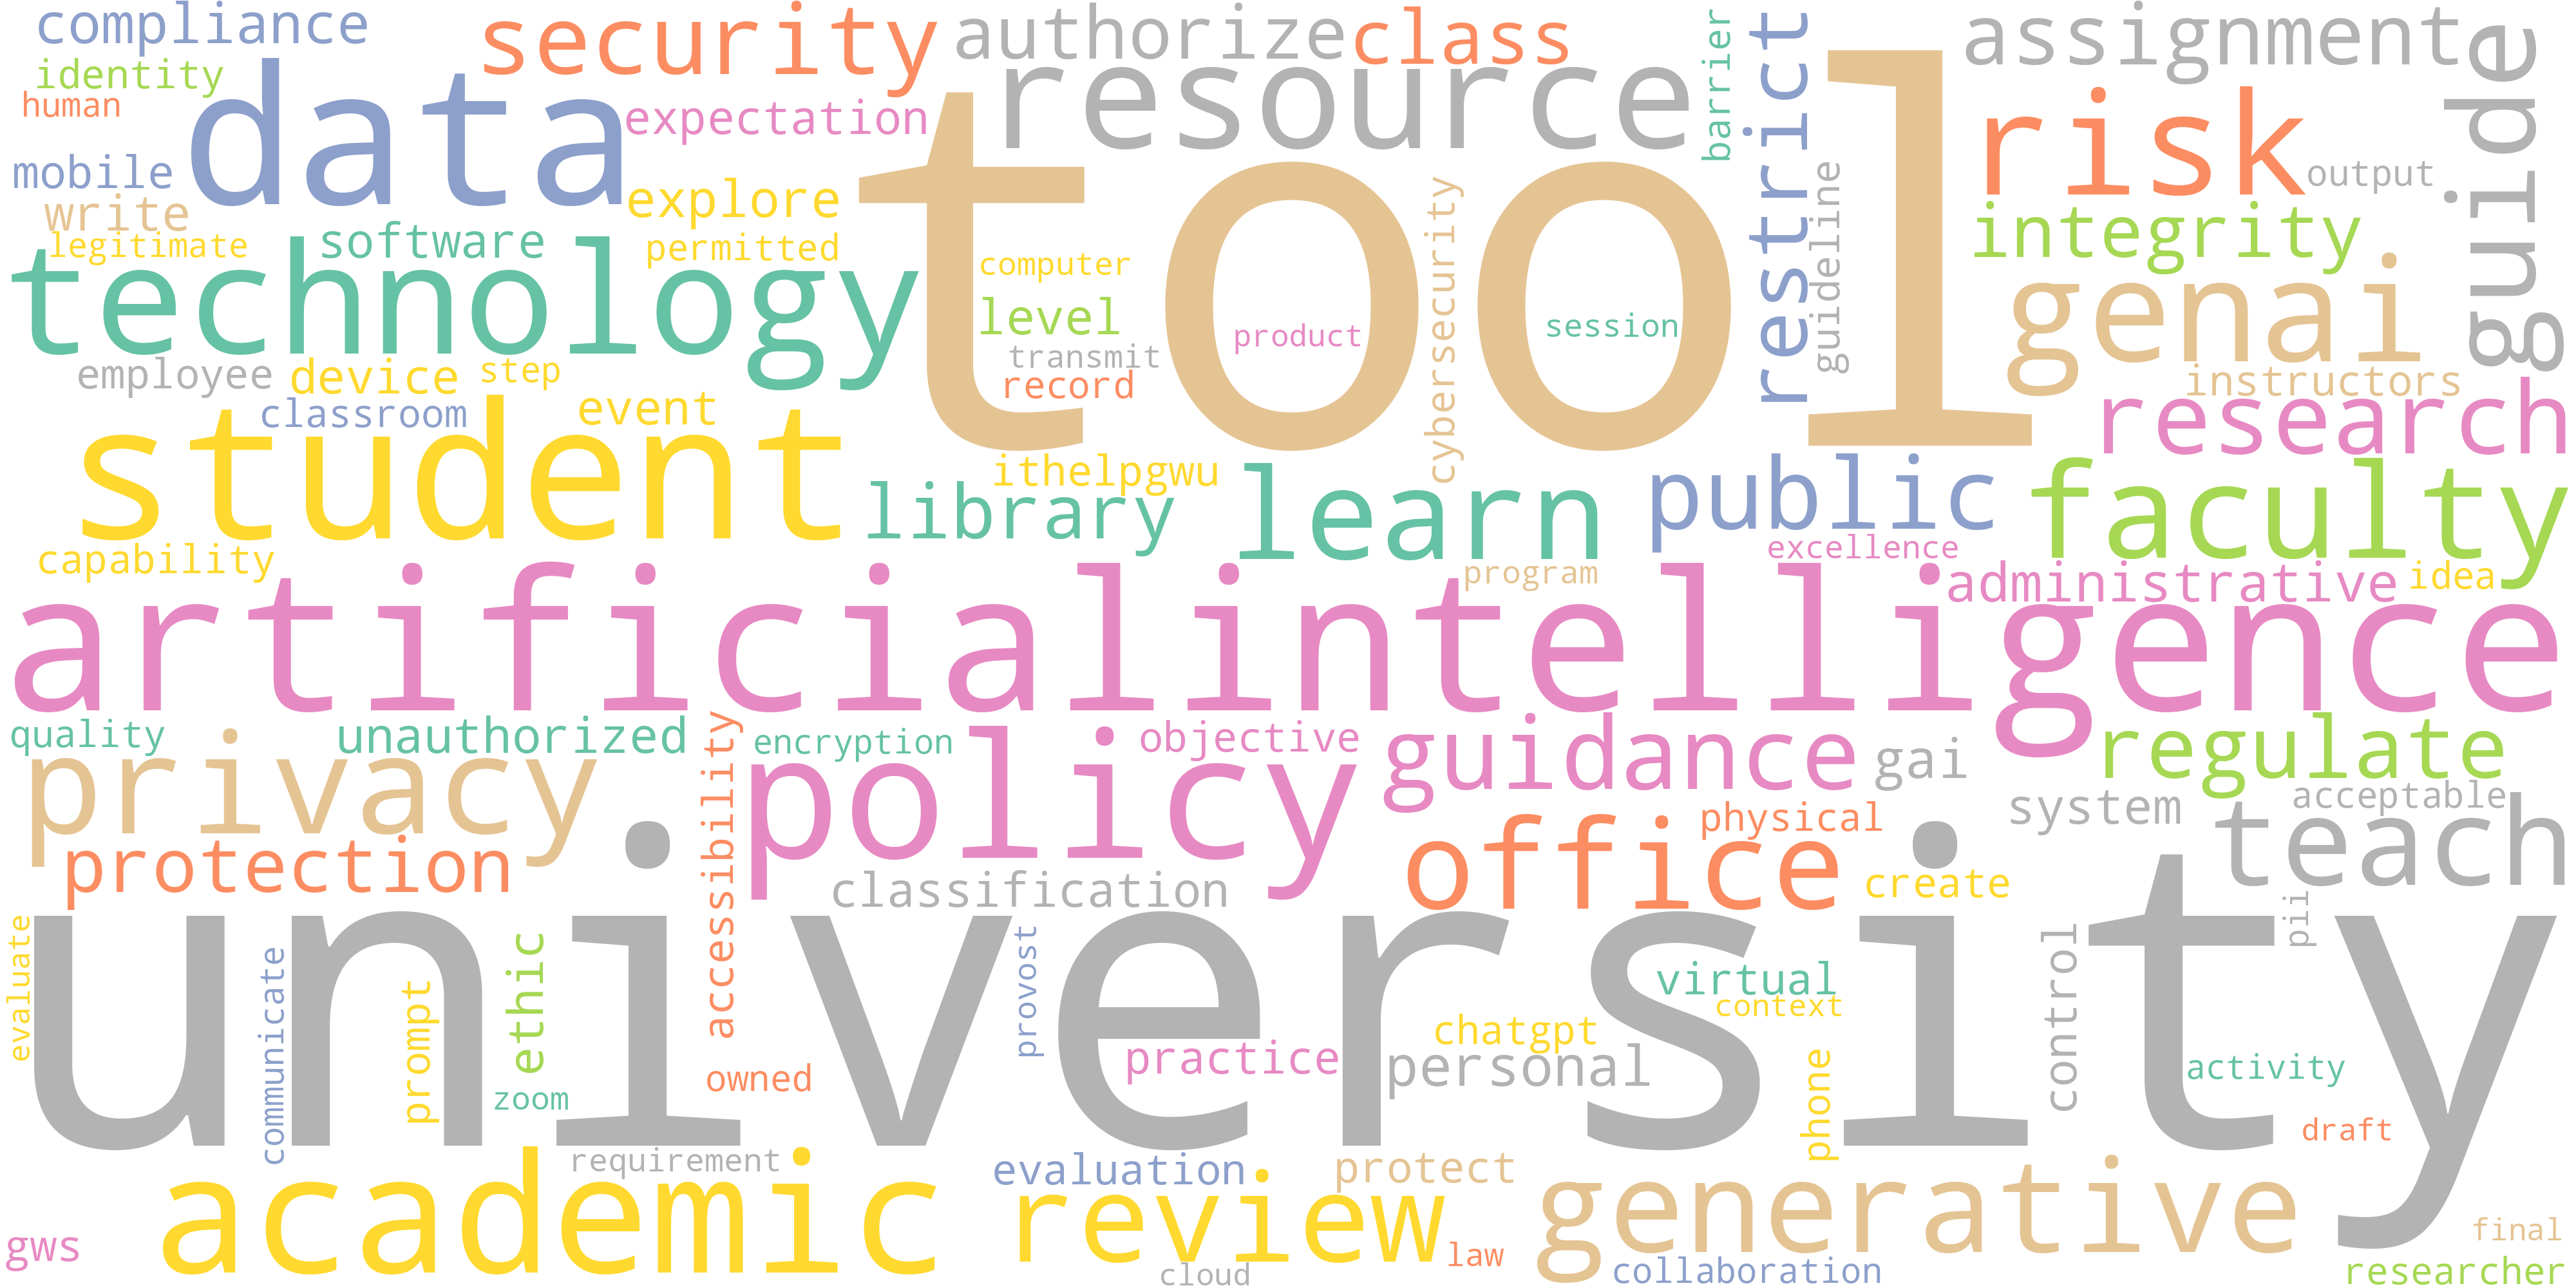
\includegraphics[width=0.87\linewidth, keepaspectratio]{existing_policy_key_word_cloud_hi_4k.png}
    \end{center}
    \caption{Top keywords across GW AI and IT policies.}
    \label{fig:gwu_wordcloud}
    \end{figure}

\end{frame}

%-------------------------
\section{3. External AI Policies}

\begin{frame}{Summary of Considered External Policies}

    \begin{itemize}
        \item Judgment-based sample of 12 large, prominent, private and public universities, e.g., Ivy Leagues and UC schools.
        \item Includes business schools, e.g., Columbia, Harvard, Stanford.
        \item Includes AI policies, AI resources, legal alerts, research guidance, staff guidance, and teaching guidance. 
        \item See Slide \ref{external_policies} for a complete listing of considered external policies. 
    \end{itemize}

\end{frame}

\subsection*{Analysis}

\begin{frame}{\small{Summary of Considered External AI Policies--Word Cloud}}

    \begin{figure}
    \begin{center}
        
\includegraphics[width=0.87\linewidth, keepaspectratio]{nongwu_policy_key_word_cloud_hi_4k.png}
    \end{center}
    \caption{Top keywords across external AI policies.}
    \label{fig:external_wordcloud}
    \end{figure}

\end{frame}

%-------------------------
\section{4. Gaps and Points of Interest}\label{gap_analysis}

\begin{frame}{Summary of Potential Gaps}

    \small

    \begin{itemize}
        \item Relative to external resources, GW could likely bolster AI policies related to:
        \begin{itemize}
            \item AI governance processes and procedures. 
            \begin{itemize}
                \item E.g., specific mechanisms for AI policy adherence and enforcement, specific roles for senior leadership, updates to code of integrity. 
            \end{itemize}
            \item GW-approved tools do not yet include AI APIs or agentic tools. 
            \item Responsible AI and AI safety.
            \begin{itemize}
                \item E.g., Specific guidance on high-risk use/misuse (nondiscrimination testing of hiring tools/malicious generation of non-consensual intimate imagery (NCII) with AI tools).
            \end{itemize}
            \item Clearer guidance on AI use in research and knowledge generation. 
                \begin{itemize} 
                \item See, e.g., USC's \href{https://libguides.usc.edu/generative-AI/home}{Using Generative AI in Research} or Columbia's \href{https://provost.columbia.edu/content/office-senior-vice-provost/ai-policy}{Generative AI Policy} (contains 33 mentions of ``research'').
            \end{itemize}  
        \end{itemize}
        \item Many GW policies and guides reference unapproved tools, e.g., ChatGPT and Claude--example syllabus statements from the Provost may need to be updated.
    \end{itemize}

\end{frame}

\begin{frame}{Summary of Points of Interest}

    \small

    \begin{itemize}
    \item AI principles: \href{https://ai.universityofcalifornia.edu/governance-transparency/}{UC} (System)
    \item AI policies: \href{https://provost.columbia.edu/content/office-senior-vice-provost/ai-policy}{Columbia} (solid focus on research), \href{https://students.business.columbia.edu/office-of-student-affairs/academic-advising-and-student-success/academic-integrity/generative-ai-policy}{Columbia Business}, \href{https://honorcode.nd.edu/generative-ai-policy-for-students-august-2023/}{Notre Dame} (student honor code example), \href{https://oercs.berkeley.edu/appropriate-use-generative-ai-tools}{UC Berkeley}
    \item Syllabus statements: \href{https://cndls.georgetown.edu/resources/syllabus-policies/ai-and-homework-support/}{Georgetown}, \href{https://provost.gwu.edu/sites/g/files/zaxdzs5926/files/2023-04/generative-artificial-intelligence-guidelines-april-2023.pdf}{GW}, \href{https://tlhub.stanford.edu/docs/course-policies-on-generative-ai-use/}{Stanford Business}, \href{https://teaching.washington.edu/course-design/ai/sample-ai-syllabus-statements/}{University of Washington}
    \item Toolkits: \href{https://docs.google.com/document/d/1hQwgSR1Caksy7Rb2LRBhLEBugDLTsuMJVLTFLgDXxu8/edit?tab=t.0}{Classroom Expectations Worksheet} (GW Libraries), \href{https://sites.google.com/view/aiassignments}{Can I Use AI?} (Prof. Ryan Watkins, GW), \href{https://cndls.georgetown.edu/resources/ai/}{Georgetown Center for New Designs in Learning and Scholarship (CNDLS)}, \href{https://tll.mit.edu/teaching-resources/course-design/gen-ai-your-course/}{MIT Teaching + Learning Lab}, \href{https://docs.google.com/document/d/1Nutviqrix6NMb1XLM2N5nLe2Q1_7JHu5aTXlnSxKCh0/edit?tab=t.0}{Student Checklist} (GW Libraries)
    \item Topic model outliers:
    \begin{itemize}
        \item \href{https://oercs.berkeley.edu/CERC-AIR}{UC Berkeley AI Risk Subcommittee}: Enterprise risk/governance vs. teaching/student guidance; potential model for an AI-specific governance mechanism.
        \item \href{https://cndls.georgetown.edu/resources/ai/}{Georgetown CNDLS}: Holistic, full-featured AI teaching toolkit.
    \end{itemize}
    \item Track GW AI tool \href{https://it.gwu.edu/ai-tools-status}{evaluation status}.
    \end{itemize}
    
\end{frame}



%-------------------------
\section{Appendices}

\subsection{A. GW Policy References}

\begin{frame}[t, allowframebreaks]{Appendix A: GW Policy References}\label{gw_policies}

\tiny

\begin{columns}

\column[t]{0.5\textwidth}

Information Technology
\begin{itemize}
    \item \href{https://it.gwu.edu/data-classification-guide}{Data Classification Guidelines}
    \item \href{https://it.gwu.edu/data-protection-guide}{Data Protection Guidelines}
    \vspace{-5pt}
    \item \href{https://it.gwu.edu/gen-ai}{Generative Artificial Intelligence}
    \begin{itemize}\tiny
        \item \href{https://it.gwu.edu/ai-guidance-and-best-practices}{AI Guidance and Best Practices}
        \item \href{https://tinyurl.com/3zvh5b47}{AI Tools and Services (Approved Tools List)}
        \item \href{https://it.gwu.edu/ai-tools-status}{AI Evaluation and Status}\\
    \end{itemize}
\end{itemize}

Libraries and Academic Innovation
\begin{itemize}
    \item \href{https://library.gwu.edu/generative-ai}{Generative Artificial Intelligence (GenAI)}
    \item \href{https://library.gwu.edu/communicating-your-genai-expectations-your-students}{Communicating GenAI Expectations to Students} (May 2025)
    \item \href{https://library.gwu.edu/deciding-appropriate-use-genai-academic-classes}{Deciding on Appropriate Use of GenAI in Classes} (May 2025)
    \item \href{https://library.gwu.edu/teaching-generative-ai}{Teaching with Generative AI}
    %\item \href{https://library.gwu.edu/users/karen-singer-freeman}{Karen Singer-Freeman} (GenAI in Teaching Lead)\\
\end{itemize}

Office of Ethics, Compliance, and Risk
\begin{itemize}
    \item \href{https://compliance.gwu.edu/acceptable-use-it-resources-policy}{Acceptable Use of IT Resources Policy} (Sept.\ 2023)
    \item \href{https://compliance.gwu.edu/cybersecurity-risk-policy}{Cybersecurity Risk Policy} (Oct.\ 2023)
    \item \href{https://compliance.gwu.edu/identity-and-access-management-policy}{Identity and Access Management (IAM) Policy} (Oct.\ 2023)
\end{itemize}

\column[t]{0.5\textwidth}

Office of the Provost
\begin{itemize}
    \vspace{-5pt}
    \item \href{https://provost.gwu.edu/guidelines-using-generative-artificial-intelligence-connection-academic-work-0}{Guidelines for Using GenAI in Academic Work} (Apr.\ 2023)
    \begin{itemize}\tiny
        \item \href{https://provost.gwu.edu/sites/g/files/zaxdzs5926/files/2023-04/generative-artificial-intelligence-guidelines-april-2023.pdf}{GenAI Guidelines (PDF)} (Apr.\ 2023)
        \item \href{https://provost.gwu.edu/sites/g/files/zaxdzs5926/files/2023-08/additional_guidance_for_generative_ai_-_august_2023.pdf}{Additional GenAI Guidance (PDF)} (Aug.\ 2023)
    \end{itemize}
\end{itemize}

Privacy Office
\begin{itemize}
    \item \href{https://privacy.gwu.edu/privacy-guidance-use-artificial-intelligence}{Privacy Guidance for Use of AI}
    \item \href{https://privacy.gwu.edu/privacy-considerations-when-using-virtual-meeting-and-collaboration-platforms}{Privacy Considerations for Virtual Platforms}
\end{itemize}

\end{columns}

\end{frame}

\subsection{B. External Policy References}

\begin{frame}[t]{Appendix B: External Policy References}\label{external_policies}
\tiny
\begin{columns}[t]

  % ---------- Left column ----------
  \begin{column}{0.48\textwidth}

Columbia University
\begin{itemize}
  \item \href{https://students.business.columbia.edu/office-of-student-affairs/academic-advising-and-student-success/academic-integrity/generative-ai-policy}{Columbia Business School, Generative AI Policy}
  \item \href{https://ctl.columbia.edu/resources-and-technology/resources/ai-tools/}{Considerations for AI Tools in the Classroom}
  \item \href{https://provost.columbia.edu/content/office-senior-vice-provost/ai-policy}{Generative AI Policy}
\end{itemize}

Georgetown University
\begin{itemize}
  \item \href{https://cndls.georgetown.edu/resources/syllabus-policies/ai-and-homework-support/}{Artificial Intelligence and Homework Support Policies}
  \item \href{https://guides.library.georgetown.edu/ai}{Artificial Intelligence (Generative) Resources}
  \item \href{https://cndls.georgetown.edu/resources/ai/}{Artificial Intelligence (AI) Toolkit (CNDLS)}
\end{itemize}

Harvard University
\begin{itemize}
  \item \href{https://www.hbs.edu/mba/handbook/standards-of-conduct/academic/Pages/chatgpt-and-ai.aspx}{Harvard Business School (HBS): Using ChatGPT and AI Tools}
  \item \href{https://registrar.gse.harvard.edu/AI-policy}{Harvard Graduate School of Education (HGSE) AI Policy}
  \item \href{https://provost.harvard.edu/guidelines-using-chatgpt-and-other-generative-ai-tools-harvard}{Guidelines for Using ChatGPT and Other Generative AI Tools}
\end{itemize}

MIT
\begin{itemize}
  \item \href{https://ist.mit.edu/ai-guidance}{Guidance for Use of Generative AI Tools}
  \item \href{https://tll.mit.edu/teaching-resources/course-design/gen-ai-your-course/}{Generative AI and Your Course}
\end{itemize}

  \end{column}

  % ---------- Right column ----------
  \begin{column}{0.48\textwidth}

Stanford University
\begin{itemize}
  \item \href{https://tlhub.stanford.edu/docs/course-policies-on-generative-ai-use/}{Stanford Graduate School of Business (GSB): Course Policies on Generative AI Use}
  \item \href{https://teachingcommons.stanford.edu/teaching-guides/artificial-intelligence-teaching-guide}{Artificial Intelligence Teaching Guide}
  \item \href{https://teachingcommons.stanford.edu/teaching-guides/artificial-intelligence-teaching-guide/creating-your-course-policy-ai}{Creating Your Course Policy on AI}
  \item \href{https://communitystandards.stanford.edu/generative-ai-policy-guidance}{Generative AI Policy Guidance}
  \item \href{https://uit.stanford.edu/security/responsibleai}{Responsible AI at Stanford}
\end{itemize}

University of California (System)
\begin{itemize}
  \item \href{https://ai.universityofcalifornia.edu/governance-transparency/}{AI Governance and Transparency}
  \item \href{https://ai.universityofcalifornia.edu/governance-transparency/applicable-law-and-policy.html}{Applicable Law and UC Policy}
  \item \href{https://www.ucop.edu/ethics-compliance-audit-services/_files/compliance/ai/ai-alert.pdf}{Legal Alert: Artificial Intelligence Tools}
\end{itemize}

UC Berkeley
\begin{itemize}
  \item \href{https://technology.berkeley.edu/AI}{AI at UC Berkeley}
\end{itemize}

UC Irvine
  \begin{itemize}
    \item \href{https://dtei.uci.edu/generative-ai/}{Generative AI for Teaching and Learning}
  \end{itemize}


  \end{column}

\end{columns}
\end{frame}

\begin{frame}[t]{Appendix B: External Policy References (cont.)}

\tiny

UCLA
\begin{itemize}
  \item \href{https://dts.ucla.edu/initiatives/ai}{Artificial Intelligence (AI)}
  \item \href{https://senate.ucla.edu/news/teaching-guidance-chatgpt-and-related-ai-developments}{Teaching Guidance for ChatGPT and Related AI Developments}
\end{itemize}

University of Notre Dame
\begin{itemize}
  \item \href{https://honorcode.nd.edu/ai-recommendations-for-instructors/}{AI Recommendations for Instructors}
  \item \href{https://ai.nd.edu/policies-and-guidelines/}{AI@ND Policies and Guidelines}
  \item \href{https://honorcode.nd.edu/generative-ai-policy-for-students-august-2023/}{Generative AI Policy for Students}
\end{itemize}

USC
\begin{itemize}
\item \href{https://libguides.usc.edu/generative-AI/home}{Using Generative AI in Research}
\end{itemize}

University of Washington
\begin{itemize}
  \item \href{https://teaching.washington.edu/course-design/ai/}{AI+Teaching}
  \item \href{https://teaching.washington.edu/course-design/ai/sample-ai-syllabus-statements/}{Sample AI Syllabus Statements}
\end{itemize}

Yale University
\begin{itemize}
  \item \href{https://ai.yale.edu/}{AI at Yale}
  \item \href{https://poorvucenter.yale.edu/AIguidance}{AI Guidelines}
  \item \href{https://yaledata.yale.edu/yale-university-ai-guidelines-staff}{AI Guidelines for Staff}
  \item \href{https://provost.yale.edu/news/guidelines-use-generative-ai-tools}{Guidelines for the Use of Generative AI Tools}
\end{itemize}

\end{frame}

\subsection{C. Methodological References}

\begin{frame}[t, allowframebreaks]{Appendix C: Methodological References}

This analysis combines qualitative review with topic modeling to surface structural similarities and gaps. Methodological references include:\\
\vspace{10pt}
\nocite{*}
\printbibliography[heading=none]

\end{frame}

\subsection{D. Topic Model Clusters}

\begin{frame}[t]{\small{Appendix D: Summary of GW AI and IT Policies--Visual Map of GW Policies}}

    \begin{figure}
    \begin{center}
        
\includegraphics[height=0.39\linewidth, keepaspectratio]{doc_clus_legend_annotated_crop.png}
    \caption{Document clusters and their representative topics for GW AI and IT policies. Large image available upon request.}
    \end{center}
    \end{figure}

\end{frame}

\begin{frame}{\small{Appendix D: Summary of GW AI and IT Policies--Visual Map Takeaways}}
\scriptsize
\vspace{5pt}
\begin{itemize}
  \item \textbf{Teaching and Student Use (Provost + Libraries):} On the left, Provost and Libraries guidance form a large cluster focused on assignments, tools, integrity, expectations, and instructor–student communication. (Labels: \texttt{Provost 1} and \texttt{Provost 2}; \texttt{Teaching with Gen AI (Libraries)}, \texttt{Communicating Expectations (Libraries)}, \texttt{Generative AI (Libraries)}, and \texttt{Deciding on Use (Libraries)}.)

  \item \textbf{Library AI Toolkit:} Within that region, the Libraries’ AI pages cluster tightly together, providing  toolkits that link AI to classes, assignments, faculty support, and concrete teaching strategies. (Labels: \texttt{Teaching with Gen AI (Libraries)}, \texttt{Communicating Expectations (Libraries)}, \texttt{Generative AI (Libraries)}, and \texttt{Deciding on Use (Libraries)}.)

  \item \textbf{IT AI Guidance, Privacy, and Meetings:} In the upper–central area, AI Guidance and Best Practice and the general Privacy Guidance documents connect AI use to data handling and personal-information protection, while a nearby Meetings cluster concentrates on virtual-meeting platforms. (Labels: \texttt{AI Guidance and Best Practice (IT)}, \texttt{Privacy Guidance: Meetings}, and \texttt{Privacy Guidance}.)

  \item \textbf{Tool Evaluation and Approved Tools:} Lower down, Tool Evaluation and Approved Tools form an operational cluster about evaluating, approving, and supporting specific tools (e.g., Zoom, chatbots) for academic use. (Labels: \texttt{Tool Evaluation (IT)} and \texttt{Approved Tools (IT)}.)

  \item \textbf{Baseline IT Risk and Data Governance:} On nearer right, Data Classification and Data Protection policies transition into Acceptable Use, Cybersecurity Risk, and IAM policies on the far right (Office of Ethics, Compliance, and Risk (OECR)), representing GW’s underlying data-governance and risk/compliance policies that AI-specific guidance builds upon. (Labels: \texttt{Data Classification (IT)} and \texttt{Data Protection (IT)}; \texttt{Acceptable Use (OECR)}, \texttt{Cybersecurity Risk (OECR)}, and \texttt{IAM (OECR)}.)
\end{itemize}

\end{frame}

\begin{frame}{\small{Appendix D: Summary of Considered External AI Policies--Visual Map of Policies}}

    \begin{figure}
    \begin{center}
        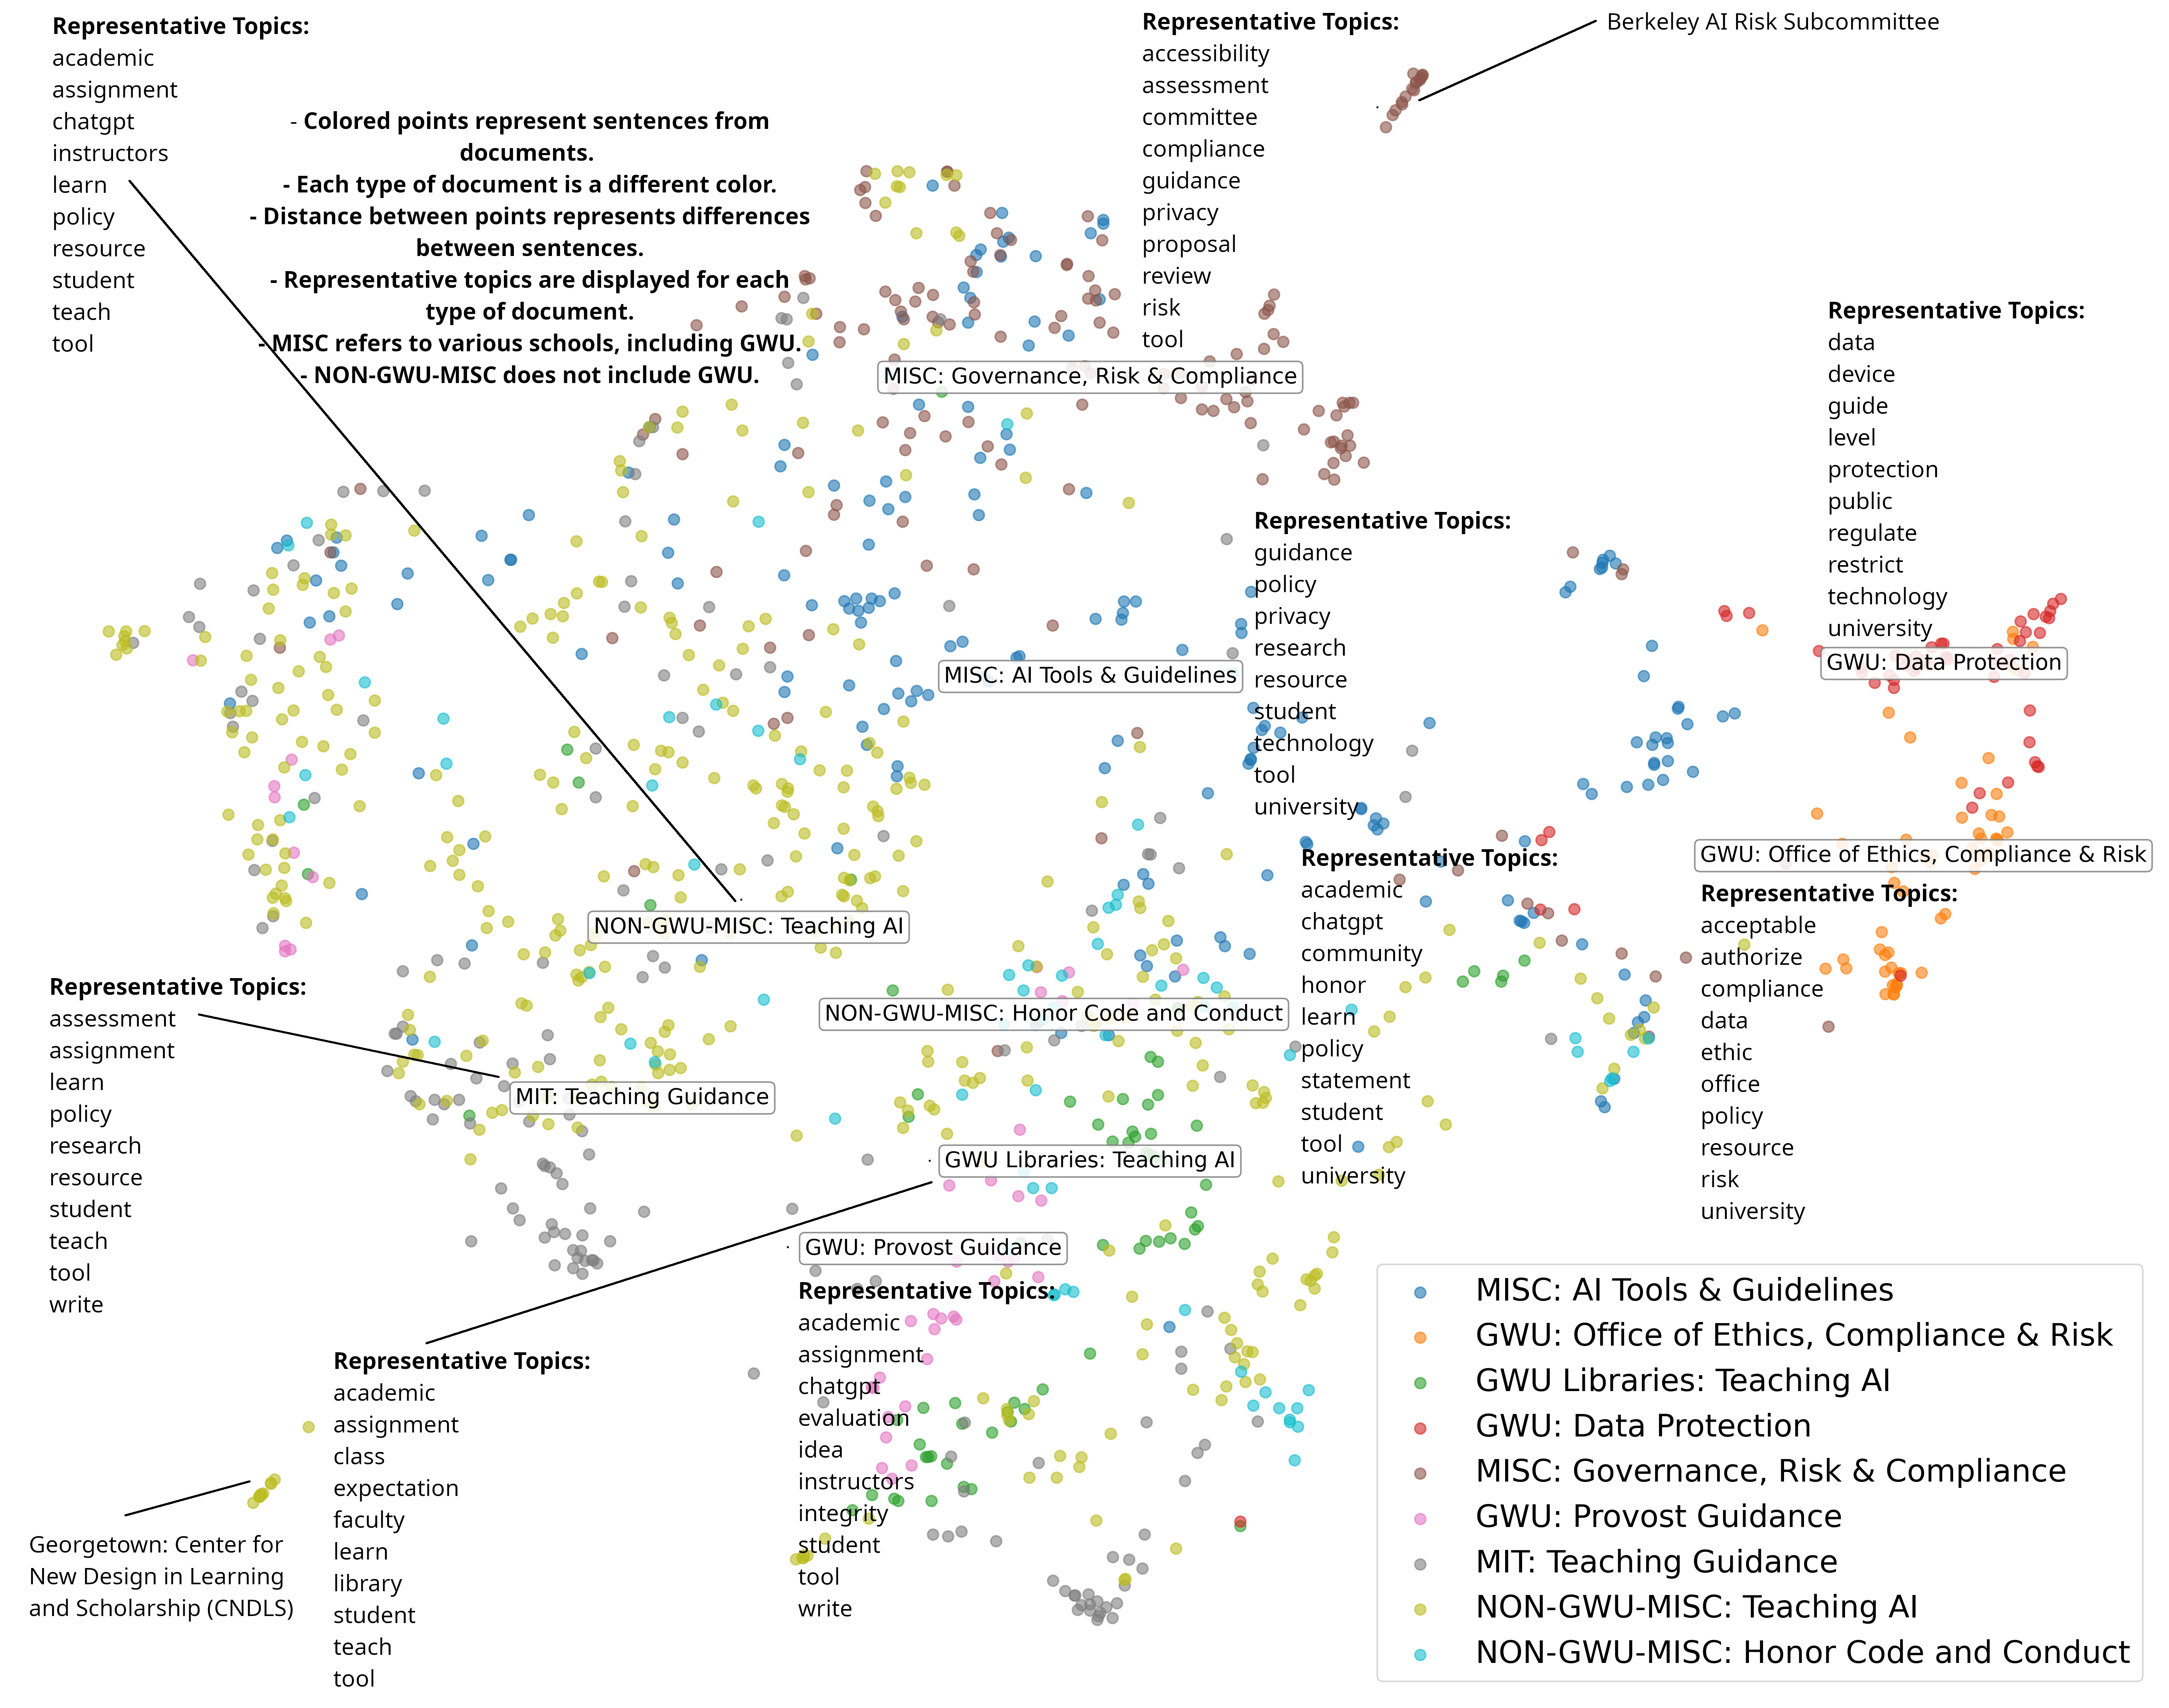
\includegraphics[height=0.4\linewidth, keepaspectratio]{doc_clus_legend_annotated_crop_nongwu.png}
    \caption{Document clusters and their representative topics for external AI policies. Large image available upon request.}
    \end{center}
    \end{figure}

\end{frame}

\begin{frame}{\small{Appendix D: Summary of Considered External AI Policies--Visual Map Takeaways}}
\scriptsize
\begin{itemize}

  \item \textbf{Governance Mechanisms:} On the upper and right sides of the map, Berkeley’s AI Risk Subcommittee and related compliance, cybersecurity, and data-protection documents--including some comparable GW risk/compliance policies--form a governance cluster that represents the most formal and centralized oversight of AI use. (Labels: \texttt{MISC: Governance, Risk, \& Compliance}, \texttt{GWU Data Protection}, \texttt{GWU Office of Ethics, Compliance, \& Risk}.)

  \item \textbf{AI Tools and Guidance:} AI guidance that focuses on tooling, and includes GW IT guidance, abuts the data protection and governance clusters in a central blob of documents. (Label: \texttt{MISC: AI Tools \& Guidance.})   
 
  \item \textbf{Honor/Integrity Codes:} An honor code/conduct cluster captures many schools’ student-facing AI rules, while GW’s provost and library guidance sits nearby but separate, emphasizing teaching, evaluation, and support rather than misconduct and sanctions. (Labels: \texttt{NON-GWU-MISC: Honor Code and Conduct}, \texttt{GWU: Provost Guidance}.)

  \item \textbf{Teaching Guidance:} A left-side blob mixes less-actionable teaching and classroom guidance. (Label: \texttt{NON-GWU-MISC: Teaching AI}.)

  \item \textbf{Actionable Teaching Tools and Support:} At the teaching-oriented lower side, MIT, Georgetown CNDLS, and GW Libraries cluster around concrete assignments, assessment, and tools, with some overlap with GW Provost documents and CNDLS standing out as the most holistic toolkit. (Labels: \texttt{GWU Libraries: Teaching AI}, \texttt{GWU: Provost Guidance}, \texttt{MIT: Teaching Guidance}.)
  
\end{itemize}
    
\end{frame}

\subsection{E. Abbreviations}

\begin{frame}[t]{Appendix E: Abbreviations}
\tiny
\renewcommand{\arraystretch}{1.2}

\begin{tabular}{ll}
\textbf{Abbreviation} & \textbf{Definition} \\
AI & Artificial Intelligence \\
API & Application Programming Interface \\
GenAI/Gen AI & Generative Artificial Intelligence \\
GW/GWU & George Washington University \\
GWSB & GW School of Business \\
IT & Information Technology \\
UC & University of California \\
UCLA & University of California, Los Angeles \\
USC & University of Southern California \\
MIT & Massachusetts Institute of Technology \\
HBS & Harvard Business School \\
HGSE & Harvard Graduate School of Education \\
GSB & Graduate School of Business (Stanford University) \\
CNDLS & Center for New Designs in Learning and Scholarship (Georgetown University) \\
IAM & Identity and Access Management \\
OECR & Office of Ethics, Compliance, and Risk \\
NCII & Non-consensual Intimate Imagery \\
\end{tabular}

\end{frame}

\end{document}
